\documentclass[oneside,14pt]{extarticle}
\usepackage{cmap}
\usepackage[utf8]{inputenc}
\usepackage[english,ukrainian]{babel}
\usepackage{graphicx}
\usepackage{geometry}
\usepackage[labelsep=period]{caption}
\usepackage{indentfirst}
\usepackage{listings}
\usepackage{float}
\usepackage{amsmath}
\usepackage{subfig}
\usepackage{tempora}
\geometry{
	a4paper,
	left=20mm,
	right=20mm,
	top=15mm,
	bottom=15mm,
}
\lstset{
	language=c,
	tabsize=4,
	keepspaces,
	showstringspaces=false,
	frame=single,
	breaklines,
	language=C,
}
\graphicspath{ {./pictures} }
\setlength{\parindent}{4em}

\newcommand\subject{Основи інтернету речей}
\newcommand\lecturer{професор кафедри ПЗ\\Фечан А.В.}
\newcommand\teacher{асистент кафедри ПЗ\\Далявський В.С.}
\newcommand\mygroup{ПЗ-42}
\newcommand\lab{2}
\newcommand\theme{Ознайомитися з особливостями роботи середовищ програмування Keil uVision та
	STM32CubeIDE}
\newcommand\purpose{Встановити взаємозв’язок між середовищем програмування та розміром і швидкістю
	виконання програмного коду}

\begin{document}
\begin{normalsize}
	\begin{titlepage}
		\thispagestyle{empty}
		\begin{center}
			\textbf{МІНІСТЕРСТВО ОСВІТИ І НАУКИ УКРАЇНИ\\
				НАЦІОНАЛЬНИЙ УНІВЕРСИТЕТ "ЛЬВІВСЬКА ПОЛІТЕХНІКА"}
		\end{center}
		\begin{flushright}
			\textbf{ІКНІ}\\
			Кафедра \textbf{ПЗ}
		\end{flushright}
		\vspace{80pt}
		\begin{center}
			\textbf{ЗВІТ}\\
			\vspace{10pt}
			до лабораторної роботи № \lab\\
			\textbf{на тему}: <<\textit{\theme}>>\\
			\textbf{з дисципліни}: <<\subject>>
		\end{center}
		\vspace{80pt}
		\begin{flushright}
			
			\textbf{Лектор}:\\
			\lecturer\\
			\vspace{28pt}
			\textbf{Виконав}:\\
			
			студент групи \mygroup\\
			Коваленко Д.М.\\
			\vspace{28pt}
			\textbf{Прийняв}:\\
			
			\teacher\\
			
			\vspace{28pt}
			«\rule{1cm}{0.15mm}» \rule{1.5cm}{0.15mm} 2024 р.\\
			$\sum$ = \rule{1cm}{0.15mm}……………\\
			
		\end{flushright}
		\vspace{\fill}
		\begin{center}
			\textbf{Львів – 2024}
		\end{center}
	\end{titlepage}
		
	\begin{description}
		\item[Тема.] \theme.
		\item[Мета.] \purpose.
	\end{description}

    \section*{\hfil Лабораторне завдання\hfil}
	\begin{enumerate}
		\item Встановити середовища STM32CubeIDE (повинно бути вже встановлено для виконання
		ЛР№1) та Keil uVision.
		\item Трансформувати індивідуальне завдання для забезпечення можливості вимірювання часу
		виконання коду(збільшити розмір коду).
		\item Створити проект згідно індивідуального завдання для борду STM32F4 Discovery з
		застоуванням середовища програмування STM32CubeIDE.
		\item Створити проект згідно індивідуального завдання для мікроконтролера STM32F407VG з
		застоуванням середовища програмування STM32CubeIDE.
		\item Створити проект згідно індивідуального завдання для мікроконтролера STM32F407VG з
		застоуванням середовища програмування Keil uVision.
		\item Проекти для мікроконтролерів наповнити кодом (можна включити переферію або додати
		файли із різними функціями та статичними змінними).
		Рекомендовано не включати важку переферію, таку як USB, Ethernet, тощо, оскільки
		згенерований код може викликати помилки збірки проекту.
		Для об’єктивності результатів рекомендовано згенерувати проект для Keil в середовищі
		STM32CubeMX.
		\item Порівняти розмір отриманого коду та час його виконання у пунктах 3-5.
		\item Оптимізувати розмір коду отриманий в п.3 шляхом вилучення зайвих автоматично
		згенерованих ділянок.
		\item Порівняти час збирання проектів з пунктів 3-5.
		\item Порівняти розміни прошивок, що генеруються середовищами згаданими в пунктах 3-5.
		\item Порівняти розміри hex файлів (можна bin).
		\item Оцінити можливість міграції проектів з stm32cudeIDE в KEIL та навпаки.
	\end{enumerate}

Вмикання по черзі червоного та синього світлодіодів, через 1 с – зеленого та жовтого
світлодіоду одночасно

\section*{\hfil Теоретичні відомості\hfil}
Keil uVision та STM32CubeIDE — це обидві IDE, призначені для розробки вбудованих систем, але вони мають різні підходи та можливості.

Keil uVision:

Переважно використовується для мікроконтролерів на базі ARM Cortex-M (STM32, LPC тощо).
Має інтеграцію з ARM MDK (Microcontroller Development Kit) для крос-компіляції під ARM процесори.
Пропонує високоякісну підтримку RTOS та зручний налагоджувач з розширеними можливостями.
Ліцензійне ПЗ, яке може бути дорогим у порівнянні з іншими альтернативами.

STM32CubeIDE:

Офіційна IDE від STMicroelectronics для мікроконтролерів STM32, заснована на Eclipse з інтеграцією CubeMX для налаштування периферії.
Повністю безкоштовна і відкриває легкий доступ до конфігурації апаратних ресурсів STM32 через CubeMX.
Пропонує широку підтримку генерації коду, включаючи HAL та LL бібліотеки для STM32.

	\section*{\hfil Хід роботи\hfil}
	
	Спочатку було встановлено середовища розробки STM32CubeIDE та Keil uVision. На початку тестування використано STM32CubeIDE для налаштування проекту на борду STM32F4 Discovery, де розроблено простий код для ввімкнення світлодіодів з інтервалом 1 секунда.
	
	Проект для STM32F4 Discovery включав зміну стану червоного, синього, зеленого та жовтого світлодіодів. Результати роботи коду були успішно продемонстровані на платі.
	
	\begin{figure}[H]
		\centering
		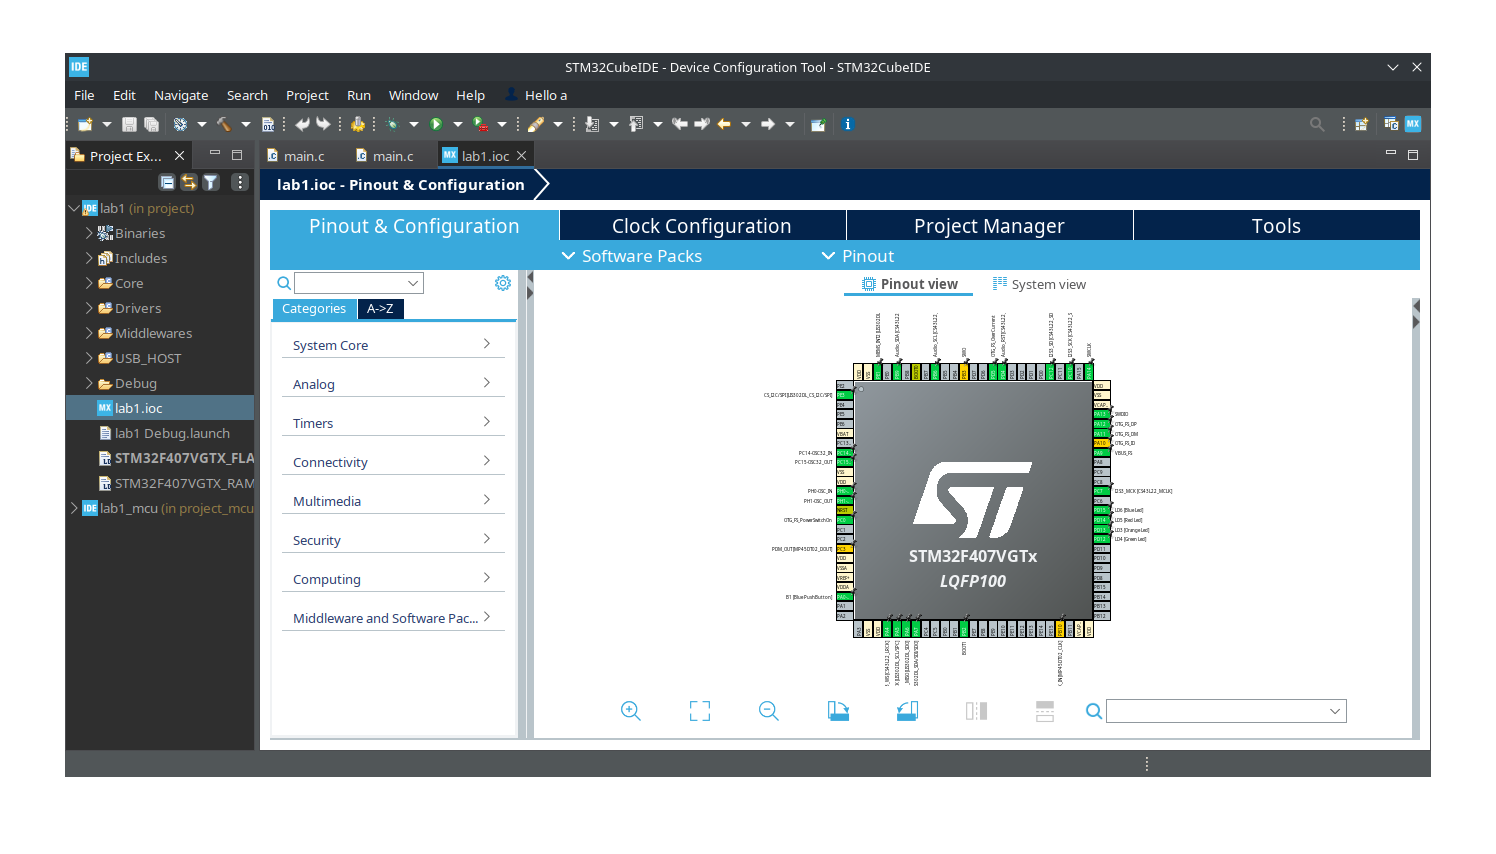
\includegraphics[scale=0.4]{1}
		\caption{Проект для борду STM32F4 Discovery}
	\end{figure}
	
	Далі, було створено проект для мікроконтролера STM32F407VG у STM32CubeIDE. Код був адаптований для іншого контролера, з урахуванням специфічних налаштувань тактованої частоти та часу затримки між зміною світлодіодів. Плата працювала коректно.
	
	\begin{figure}[H]
		\centering
		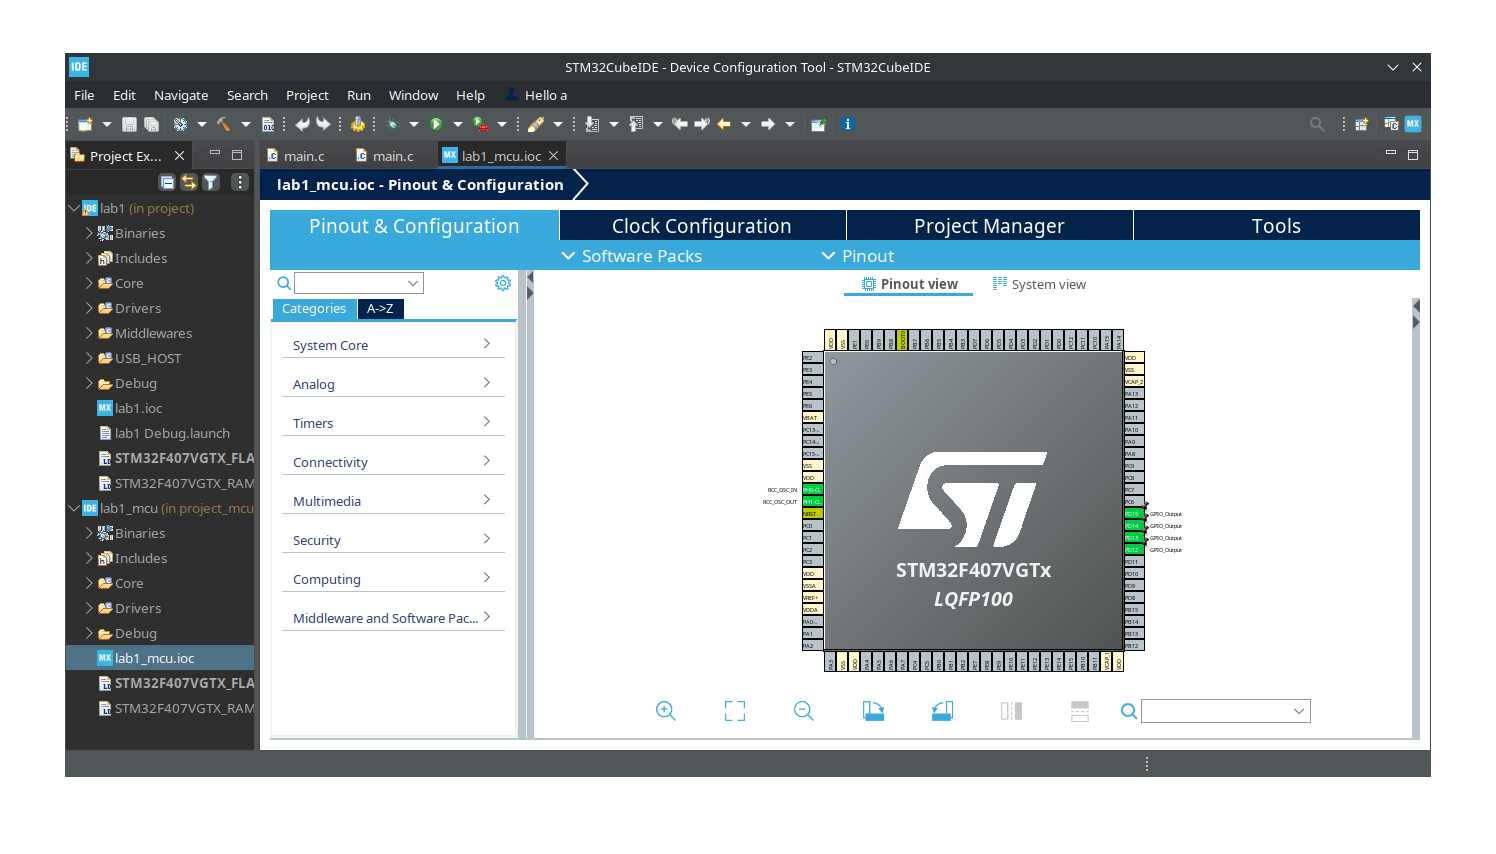
\includegraphics[scale=0.4]{2}
		\caption{Проект для борду мікроконтролера STM32F407VG}
	\end{figure}
	
	Після цього проекти було перенесено у середовище Keil uVision. За допомогою STM32CubeMX було згенеровано початковий код для Keil, що значно спростило процес міграції. Проект працював ідентично з мінімальними змінами у коді.
	
	\begin{figure}[H]
		\centering
		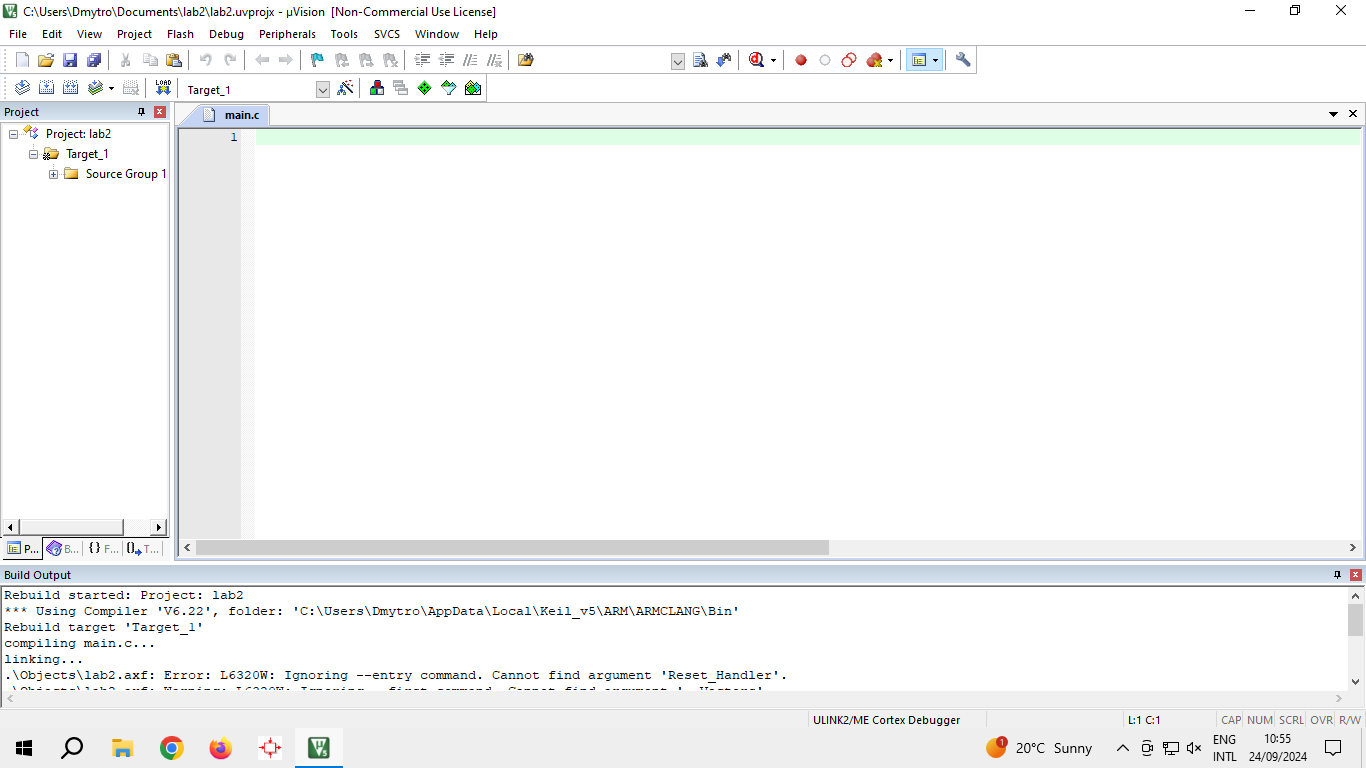
\includegraphics[scale=0.4]{3}
		\caption{Проект для борду мікроконтролера STM32F407VG}
	\end{figure}
	
	Порівняння часу компіляції та розміру hex-файлів для двох середовищ показало, що Keil uVision генерує трохи менший за розміром файл, але час компіляції для борду становить 2.9 секунди а для мікроконтролера 1.8 секунди. 
	
	\section*{\hfil Висновки\hfil}
	У результаті виконання лабораторної роботи було успішно створено та протестовано проекти для двох різних плат — STM32F4 Discovery та STM32F407VG — у середовищах STM32CubeIDE та Keil uVision. Перенесення проектів між середовищами відбулося без значних проблем завдяки використанню STM32CubeMX. Проекти працювали коректно на обох платформах, а порівняння розміру коду та часу його виконання виявило мінімальні відмінності.
		    
\end{normalsize}
\end{document}
